We know that mining is based on SHA256 so, in this part, we'll see different techniques (inspired by \cite{broken_crypto_primitives}) to defeat traditional mining if SHA256 is broken.

\section{Pre-image with fixed Merkle root}

First, we analyze the probability for an attacker with a pre-image oracle to break mining, i.e. to get a high probability of solving the PoW before the other nodes in the network.

If we suppose we can have a pre-image oracle for SHA256, then we will be able to build an oracle for $H_M(x) = SHA256(SHA256(x))$ by applying the first oracle twice.

	\subsection{Input set of $H_M$}

As explained before, a miner applies the hashing operation $H_M(x)$ to the block header. A classic miner only controls the value of the nonce but an attacker will try to control more. \newline

The version, the previous block's hash and the Merkle root are fixed fields. \newline

For the time field, the system allows a range of 7200 seconds around the current time. So, over the 32 bits dedicated to this field, an attacker will be able to control about 13 bits.

For the target, the protocol will check if the target value is at most the one defined by the consensus of the network, this means the attacker can control about 28 bits.

For the nonce, like any miner, the attacker can control the 32 bits allowed to it. \newline

The block header's size is $4 + 32 + 32 + 4 + 4 + 4 = 80$ bytes $ = 640$ bits.

An attacker can control $b = 13 + 28 + 32 = 73$ bits on the input value, which means he has $2^b$ possibilities to call the hash function $H_M$.

	\subsection{Output set of $H_M$}

The result of $H_M$ is a hash from SHA256, so it has a length of $n = 256$ bits and there are $2^n$ possibilities of outputs. \newline

Then, in order to fulfill the condition given by the target, the hash needs to start with a specific number of zeros, let's note d zeros.

In reality, matching with the coefficient may require more effort (see \ref{appendixTarget} for more details). \newline

This means that there are $2^{n-d}$ hashes lower than the target.

	\subsection{Probability of breaking mining}


By calling $H_M$, one has a probability of $\frac{2^{n-d}}{2^n}$ to get a valid hash.

That way, we can get the number of correct pre-images i.e in the input set, how many inputs will end as a correct hash.

\begin{equation}
proba\_of\_correct\_hash \times \#possible\_inputs = \frac{2^{n-d}}{2^n} \times 2^b = 2^{b-d}
\end{equation}
\newline

\begin{figure}[ht]
\centering
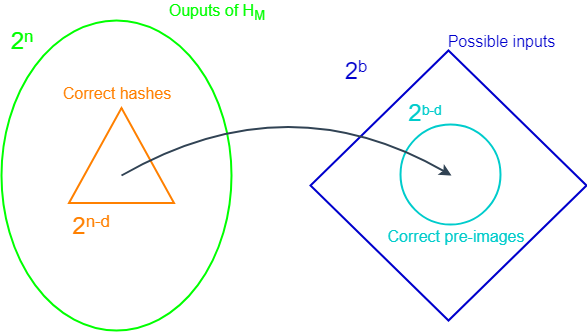
\includegraphics[width=8cm]{Figures/probaSuccess}
\caption{Probability of getting a correct pre-image}
\end{figure}
\medskip

In his attack attempt, the attacker queries the pre-image oracle for specific target hashes. So he will choose a correct hash (triangle set) and hope that the output is one of the correct pre-images. This is the probability that he gets an accepted pre-image.

\begin{equation}
\frac{\#pre-images}{\#accepted\_outputs} = \frac{2^{b-d}}{2^{n-d}} = 2^{b-n}
\end{equation}
\newline

Then, to get the real probability of success, we need to add a constraint on the number of queries allowed to the attacker. Because, otherwise, the attack won't be faster than traditional mining. So let's consider the attacker can query the oracle $2^a$ times.

\begin{equation}
P_{success} = 2^a \times 2^{b-n} = 2^{a + b - n}
\end{equation}
\newline

Finally, we can estimate this probability of success. Let's take $a = 80$ so the attacker has $2^{80}$ tries (above this value, he may need more than 10 minutes to complete his attack). So, we have $P_{success} = 2^{80+73-256} = 2^{-103} \approx 10^{-32}$, which is completely negligible.

Then, we can conclude that having a simple pre-image oracle doesn't help to break mining.
